\section{Handling conflicts}
\begin{frame}[fragile]
  \slidetitle
  This section covers the following topics:
  \begin{itemize}
    \item Solve merge conflicts
    \item Solve rebase conflicts
    \item Using diff tools
    \item 3 way merge
  \end{itemize}
\end{frame}

\subsection{Prepare a merge conflict}
\begin{frame}[fragile]
  \subslidetitle
  Switch to the master branch
  \begin{lstlisting}
(*\textcolor[HTML]{18B2B2}{(oldversion)}*) $ (*\textcolor[HTML]{0000AA}{git switch master}*)
\end{lstlisting}
  Implement the change in \cmd{moon.js} following this diff:
  \begin{lstlisting}
(*\textcolor[HTML]{18B2B2}{@@ -4,7 +4,7 @@}*)
// create moons
 new Moon("white");
(*\textcolor[HTML]{AA0000}{-}*)(*\textcolor[HTML]{AA0000}{new Moon("green");}*)
(*\textcolor[HTML]{00AA00}{+}*)(*\textcolor[HTML]{00AA00}{new Moon("red");}*)

// Function to setup the scene for our awesome moons :)
\end{lstlisting}

  Commit your changes on master:
  \begin{lstlisting}
(*\textcolor[HTML]{18B2B2}{(master)}*) $ (*\textcolor[HTML]{0000AA}{git commit -a -m "change the green moon to red"}*)
\end{lstlisting}

\end{frame}

\subsection{Prepare a merge conflict}
\begin{frame}[fragile]
  \subslidetitle

  Switch to the branch third-moon:
  \begin{lstlisting}
(*\textcolor[HTML]{18B2B2}{(master)}*) $ (*\textcolor[HTML]{0000AA}{git switch third-moon}*)
\end{lstlisting}

  Add a comment to the green moon like defined in the following diff:
  \begin{lstlisting}
(*\textcolor[HTML]{18B2B2}{@@ -4,7 +4,7 @@}*)
// create moons
 new Moon("white");
(*\textcolor[HTML]{AA0000}{-}*)(*\textcolor[HTML]{AA0000}{new Moon("green");}*)
(*\textcolor[HTML]{00AA00}{+}*)(*\textcolor[HTML]{00AA00}{new Moon("green"); // the moon was sooo green!}*)

// Function to setup the scene for our awesome moons :)
\end{lstlisting}

  Commit your changes:
  \begin{lstlisting}
(*\textcolor[HTML]{18B2B2}{(third-moon)}*) $ (*\textcolor[HTML]{0000AA}{git commit -a -m "comment on green moon"}*)
\end{lstlisting}
\end{frame}

\subsection{Prepare a merge conflict}
\begin{frame}[fragile]
  \subslidetitle

  Let's merge the third-moon branch to master:
  \begin{lstlisting}
(*\textcolor[HTML]{18B2B2}{(third-moon)}*) $ (*\textcolor[HTML]{0000AA}{git switch master}*)
Switched to branch 'master'
Your branch is ahead of 'origin/master' by 11 commits.
  (use "git push" to publish your local commits)

(*\textcolor[HTML]{18B2B2}{(master)}*) $ (*\textcolor[HTML]{0000AA}{git merge third-moon}*)
Auto-merging moon.js
CONFLICT (content): Merge conflict in moon.js
Automatic merge failed; fix conflicts and then commit the result.
\end{lstlisting}
  \centerline{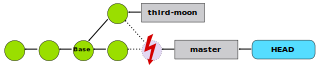
\includegraphics{assets/diagrams/merge-conflict.pdf}}
  \vspace{0.5em}
  Here we go, our first conflict, keep calm, do not panic, we are using \cmd{git}!
\end{frame}

\subsection{Displaying conflicts}
\begin{frame}[fragile]
  \subslidetitle

  First we want to display the conflicting file with \cmd{git difftool}:
  \begin{lstlisting}
(*\textcolor[HTML]{18B2B2}{(master|MERGING)}*) $ (*\textcolor[HTML]{0000AA}{git difftool}*)
diff --cc moon.js
index 72886cb,861507e..0000000
--- a/moon.js
+++ b/moon.js
(*\textcolor[HTML]{18B2B2}{@@@ -4,7 -4,7 +4,11 @@@}*)
  // create moons
  new Moon("white");
(*\textcolor[HTML]{00AA00}{++}*)(*\textcolor[HTML]{00AA00}{<<<<<<< HEAD}*)
(*\textcolor[HTML]{00AA00}{+}*) (*\textcolor[HTML]{00AA00}{new Moon("red");}*)
(*\textcolor[HTML]{00AA00}{++}*)(*\textcolor[HTML]{00AA00}{=======}*)
(*\textcolor[HTML]{00AA00}{+}*) (*\textcolor[HTML]{00AA00}{new Moon("green"); // the moon was sooo green!}*)
(*\textcolor[HTML]{00AA00}{++}*)(*\textcolor[HTML]{00AA00}{>>>>>>> third-moon}*)

// Function to setup the scene for our awesome moons :)
\end{lstlisting}
\end{frame}

\subsection{Resolving conflicts}
\begin{frame}[fragile]
  \subslidetitle
  Use \cmd{git mergetool} to open an external merge tool like kdiff3 or vimdiff to resolve a conflict:

  \begin{lstlisting}
(*\textcolor[HTML]{18B2B2}{(master|MERGING)}*) $ (*\textcolor[HTML]{0000AA}{git mergetool}*)
Merging:
moon.js

Normal merge conflict for 'moon.js':
  {local}: modified file
  {remote}: modified file
\end{lstlisting}

\end{frame}

\subsection{Resolving conflicts}
\begin{frame}[fragile]
  \subslidetitle
  The program \cmd{kdiff3} allows to perform a three way merge:
  \\
  \vspace{1em}
  \centerline{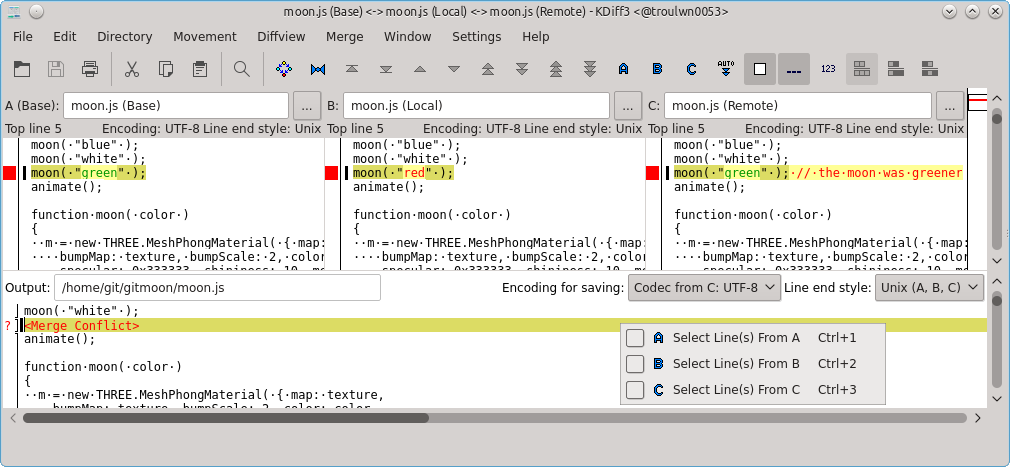
\includegraphics[width=10.5cm]{../assets/images/kdiff3.png}}

  \vspace{1em}
  Let's right-click on the conflict line and select \textbf{B}.
  \\Then, save and quit the program.
\end{frame}

\subsection{Finishing a merge}
\begin{frame}[fragile]
  \subslidetitle
  The \cmd{git status} gives some hints how to finalize the merge conflict resolution:
  \begin{lstlisting}
(*\textcolor[HTML]{18B2B2}{(master|MERGING)}*) $ (*\textcolor[HTML]{0000AA}{git status}*)
On branch master
Your branch is ahead of 'origin/master' by 11 commits.
  (use "git push" to publish your local commits)
All conflicts fixed but you are still merging.
  (use "git commit" to conclude merge)

Untracked files:
  (use "git add <file>..." to include in what will be committed)

        (*\textcolor[HTML]{AA0000}{moon.js.orig}*)

nothing added to commit but untracked files present (use "git add" to track)
\end{lstlisting}
\end{frame}

\subsection{Finishing a merge}
\begin{frame}[fragile]
  \subslidetitle

  Just use \cmd{git commit} to finish the merge, this will automatically open the text editor:
  \begin{lstlisting}
(*\textcolor[HTML]{18B2B2}{(master|MERGING)}*) $ (*\textcolor[HTML]{0000AA}{git commit}*)
Merge branch 'third-moon' into master
# Conflicts:
#       moon.js
\end{lstlisting}
  Save and quit the editor.
  \\
  \vspace{1em}
  You successfully resolved you first conflict with git, not so difficult !?
  \\
  \vspace{1em}
  Note: in order to remove temprorary files (*.orig) use the following \cmd{git clean -f} command.

\end{frame}

\subsection{Preparing rebase conflict}
\begin{frame}[fragile]
  \subslidetitle

  Create a new \cmd{death-star} branch:
  \begin{lstlisting}
(*\textcolor[HTML]{18B2B2}{(master)}*)$ (*\textcolor[HTML]{0000AA}{git switch -c death-star master}*)
Switched to a new branch 'death-star'
\end{lstlisting}

  Implement the change in \cmd{moon.js} following this diff:

  \begin{lstlisting}
(*\textcolor[HTML]{AA0000}{-}*)(*\textcolor[HTML]{AA0000}{new Moon("white");}*)
(*\textcolor[HTML]{00AA00}{+}*)(*\textcolor[HTML]{00AA00}{new Moon("black");}*)
 new Moon("red");
\end{lstlisting}

  Commit the change:
  \begin{lstlisting}
(*\textcolor[HTML]{18B2B2}{(death-star)}*)$ (*\textcolor[HTML]{0000AA}{git commit -a -m "add death-star"}*)
[death-star 2670288] add death-star
 1 file changed, 1 insertion(+), 1 deletion(-)
\end{lstlisting}
\end{frame}

\subsection{Preparing rebase conflict}
\begin{frame}[fragile]
  \subslidetitle
  Change to the master branch:
   \begin{lstlisting}
(*\textcolor[HTML]{18B2B2}{(death-star)}*)$ (*\textcolor[HTML]{0000AA}{git switch master}*)
\end{lstlisting}

  Modify the moon.js file accordingly:
  \begin{lstlisting}
(*\textcolor[HTML]{AA0000}{-}*)(*\textcolor[HTML]{AA0000}{new Moon("white");}*)
(*\textcolor[HTML]{00AA00}{+}*)(*\textcolor[HTML]{00AA00}{new Moon("white"); // as snow}*)
 new Moon("red");
\end{lstlisting}

  Commit the change:
  \begin{lstlisting}
(*\textcolor[HTML]{18B2B2}{(master)}*)$ (*\textcolor[HTML]{0000AA}{git commit -a -m "snow white comment"}*)
[master 9307b0a] snow white comment
 1 file changed, 1 insertion(+), 1 deletion(-)
\end{lstlisting}
  Change to the death-star branch:
   \begin{lstlisting}
(*\textcolor[HTML]{18B2B2}{(death-star)}*)$ (*\textcolor[HTML]{0000AA}{git switch death-star}*)
\end{lstlisting}
\end{frame}

\subsection{Rebasing with conflict}
\begin{frame}[fragile]
  \subslidetitle
  \begin{lstlisting}
(*\textcolor[HTML]{18B2B2}{(death-star)}*)$ (*\textcolor[HTML]{0000AA}{git rebase master}*)
First, rewinding head to replay your work on top of it.
Applying: add death-star
Using index info to reconstruct a base tree...
M       moon.js
Falling back to patching base and 3-way merge...
Auto-merging moon.js
CONFLICT (content): Merge conflict in moon.js
error: Failed to merge in the changes.
Patch failed at 0001 add death-star
\end{lstlisting}

  \vspace{1em}
  \centerline{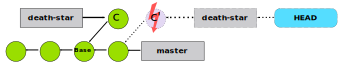
\includegraphics{assets/diagrams/rebase-conflict.pdf}}
\end{frame}

\subsection{Display conflict}
\begin{frame}[fragile]
  \subslidetitle
  First we want to display the conflicting file with \cmd{git difftool}:
  \begin{lstlisting}
(*\textcolor[HTML]{18B2B2}{(death-star|REBASE 1/1)}*) $ (*\textcolor[HTML]{0000AA}{git difftool}*)
diff --cc moon.js
index 72886cb,861507e..0000000
--- a/moon.js
+++ b/moon.js
(*\textcolor[HTML]{18B2B2}{@@@ -4,7 -4,7 +4,11 @@@}*)
(*\textcolor[HTML]{00AA00}{++}*)(*\textcolor[HTML]{00AA00}{<<<<<<< d5d25c1555e1137d3ecd3bf335d3ac3515605bf4}*)
(*\textcolor[HTML]{00AA00}{+}*) (*\textcolor[HTML]{00AA00}{new Moon("white"); // as snow}*)
(*\textcolor[HTML]{00AA00}{++}*)(*\textcolor[HTML]{00AA00}{=======}*)
(*\textcolor[HTML]{00AA00}{+}*) (*\textcolor[HTML]{00AA00}{new Moon("black");}*)
(*\textcolor[HTML]{00AA00}{++}*)(*\textcolor[HTML]{00AA00}{>>>>>>> add death-star}*)

\end{lstlisting}
\end{frame}

\subsection{Resolve rebase conflict}
\begin{frame}[fragile]
  \subslidetitle
  Resolve the conflict editing the \cmd{moon.js} file:

  \begin{lstlisting}
(*\textcolor[HTML]{AA0000}{-}*)(*\textcolor[HTML]{AA0000}{<<<<<<< d5d25c1555e1137d3ecd3bf335d3ac3515605bf4}*)
(*\textcolor[HTML]{AA0000}{-}*)(*\textcolor[HTML]{AA0000}{new Moon("white"); // as snow}*)
(*\textcolor[HTML]{AA0000}{-}*)(*\textcolor[HTML]{AA0000}{=======}*)
 new Moon("black");
(*\textcolor[HTML]{AA0000}{-}*)(*\textcolor[HTML]{AA0000}{>>>>>>> add death-star}*)
\end{lstlisting}

  \vspace{1em}
  Use \cmd{git add} to stage the changes:
  \begin{lstlisting}
(*\textcolor[HTML]{18B2B2}{(death-star|REBASE 1/1)}*) $ (*\textcolor[HTML]{0000AA}{git add moon.js}*)
\end{lstlisting}
%\end{frame}

%\subsection{Finish rebasing}
%\begin{frame}[fragile]
  %\subslidetitle
  Continue the rebase:
  \begin{lstlisting}
(*\textcolor[HTML]{18B2B2}{(death-star|REBASE 1/1)}*) $ (*\textcolor[HTML]{0000AA}{git rebase --continue}*)
Applying: add death-star
\end{lstlisting}
\end{frame}

\subsection{Summary}
\begin{frame}[fragile]
\subslidetitle
  What we've learned in this chapter:
  \begin{itemize}
    \item Why conflicts happen
    \item How to resolve conflicts
  \end{itemize}
\end{frame}
